%!TeX root=../main.tex

\begin{figure}[ht!]
\vskip -0.05in % useful knobs to optimize layout
    \centering        
    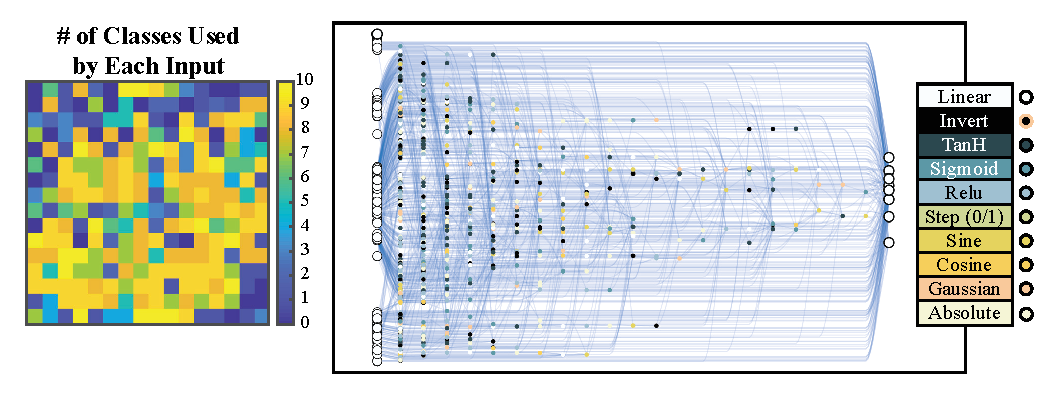
\includegraphics[width=1.0\textwidth]{img/champ_mnist_reduce_small.pdf}   
    %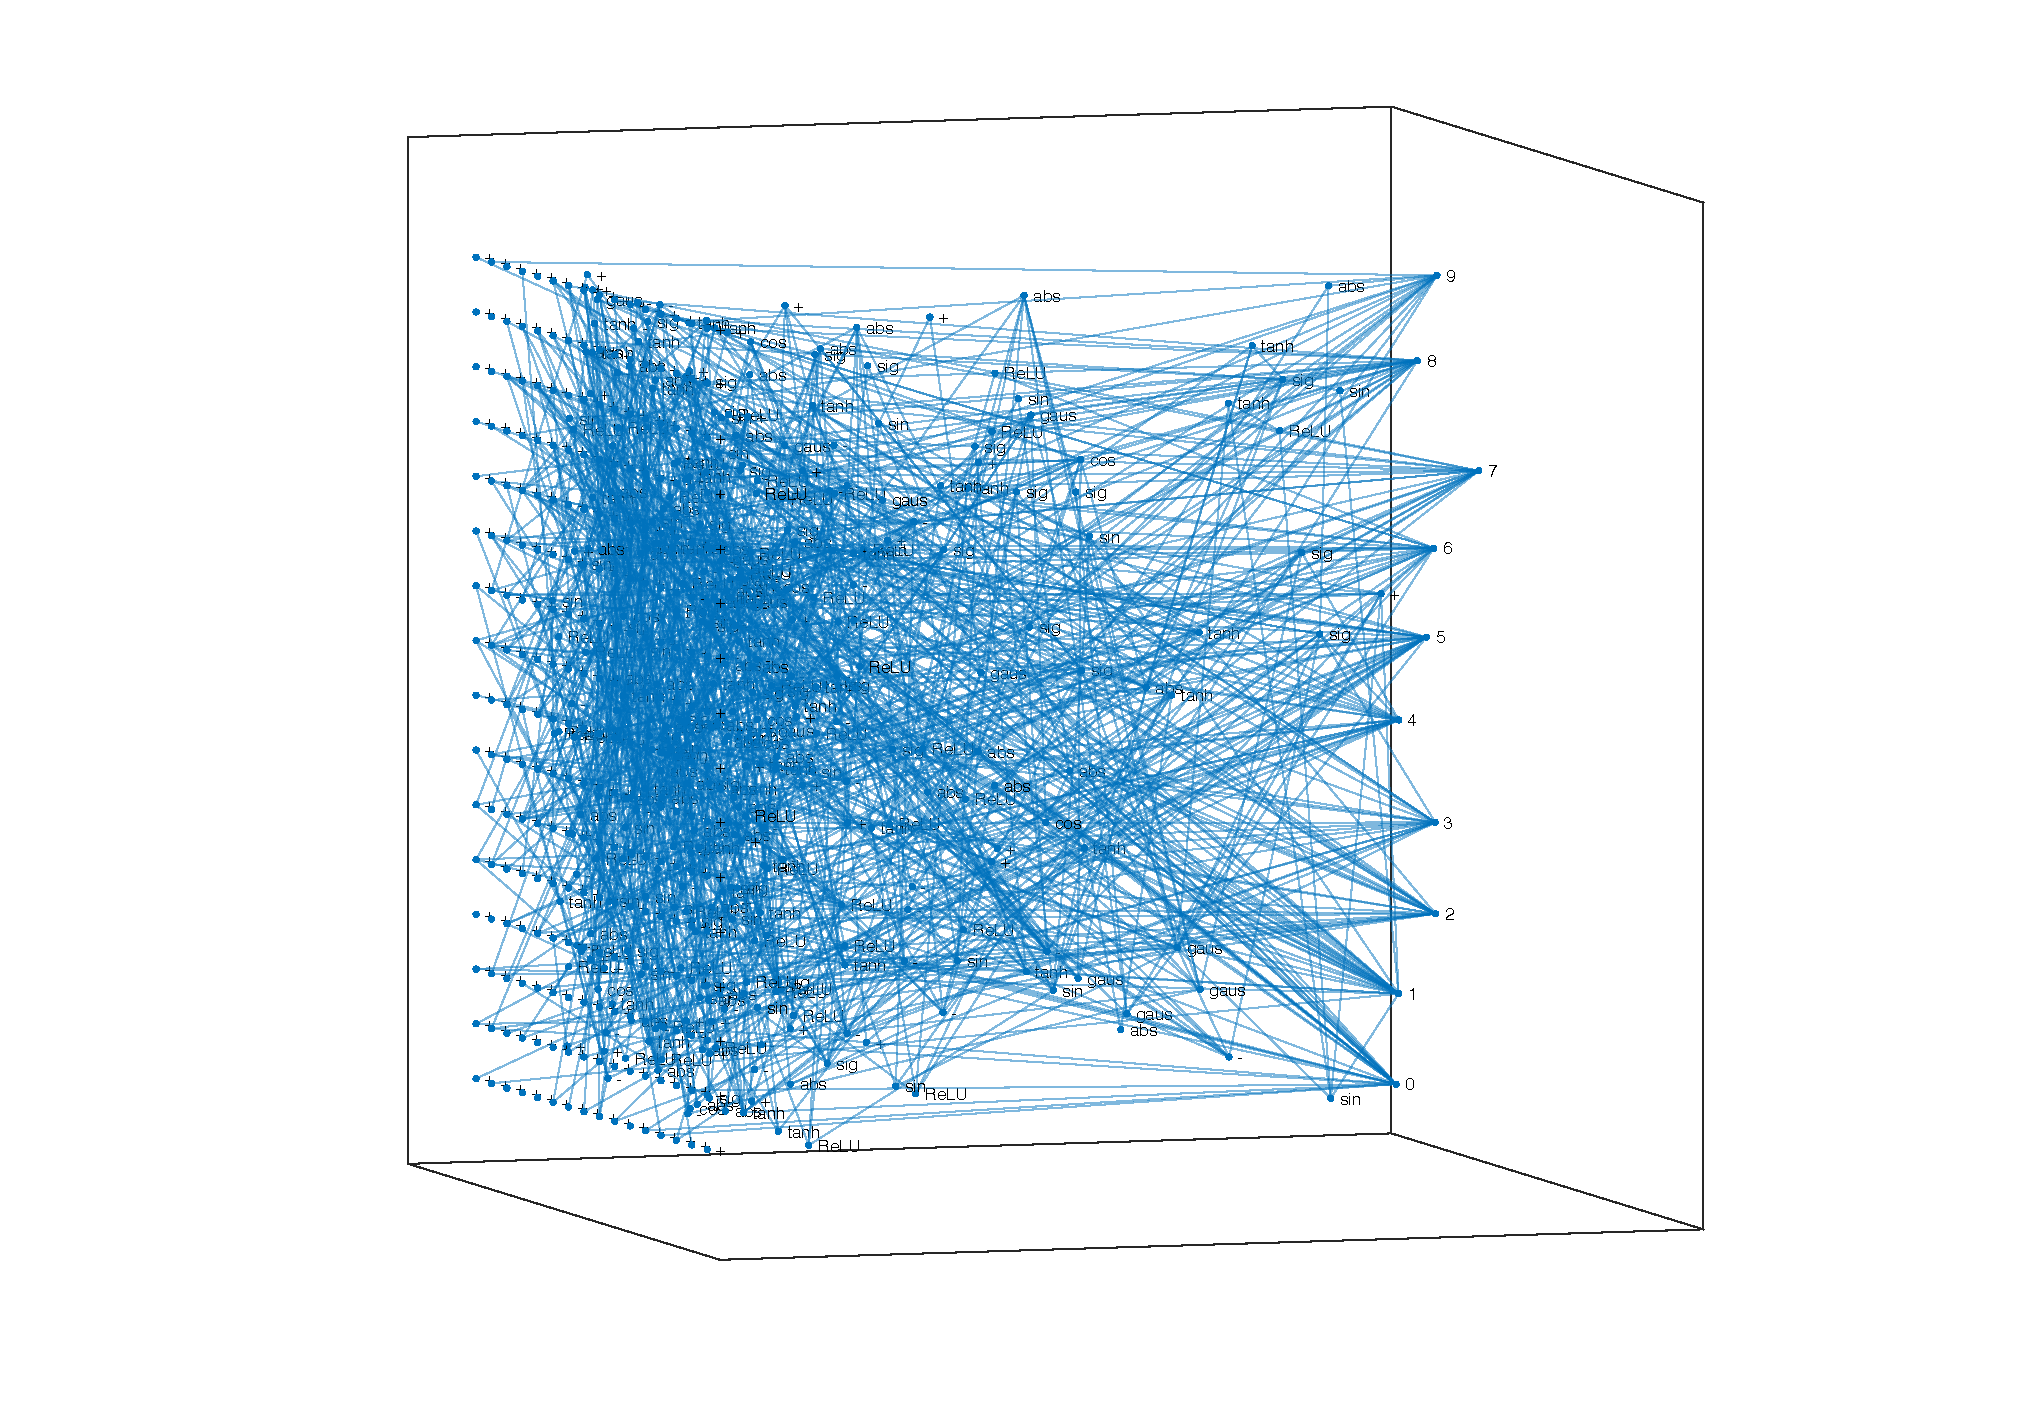
\includegraphics[width=0.45\textwidth]{supplemental/mnist_data/champ_mnist_net.pdf}   
    %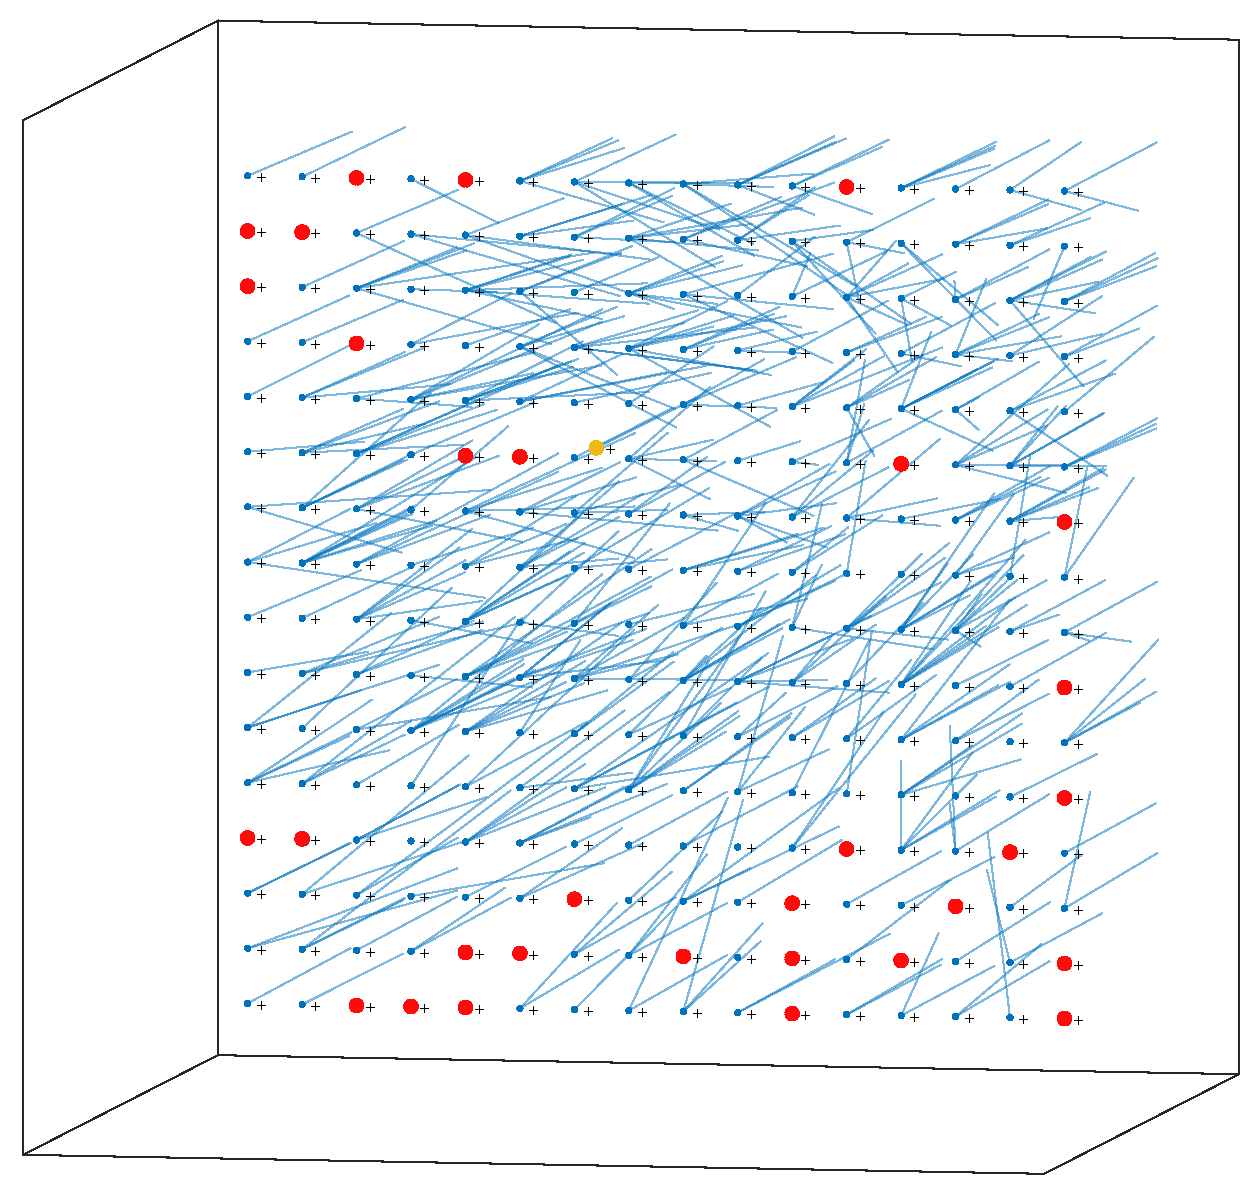
\includegraphics[width=0.45\textwidth]{supplemental/mnist_data/champ_mnist_net_input.pdf}  
\vskip -0.05in % useful knobs to optimize layout
    \caption      
    {     
	\textit{MNIST classifier network (1849 connections)}
	\newline
	Not all neurons and connections are used to predict each digit. Starting from the output connection for a particular digit, we can trace the sub-network and also identify which part of the input image is used for classifying each digit. Please refer to the \href{\websiteurl}{supplementary website} for more detailed visualizations. 
    }         
    \label{fig:mnistfull}
\vskip -0.15in % useful knobs to optimize layout
\end{figure}
